% sets document class
\documentclass[12pt, onecolumn, oneside, a4paper]{report}

% latex metadatas
% margin settings
\usepackage[top=3cm,bottom=2.5cm,left=4cm,right=2.5cm]{geometry}

% float
\usepackage{float}

% hypenation
\usepackage[none]{hyphenat}

% bahasa indo
\usepackage[bahasai]{babel}
\usepackage{csquotes}

% math support with Times font
\usepackage{mathptmx}

% datetime
\usepackage{datetime}

% biblatex
\usepackage[style=authoryear, backend=biber]{biblatex}
\addbibresource{references/paper.bib}
\addbibresource{references/website.bib}
\addbibresource{references/book.bib}

% glossary
\usepackage{glossaries}
% \makeglossaries

% \newglossaryentry{latex}
% {
%     name=latex,
%     description={Is a markup language specially suited 
%     for scientific documents}
% }

% \newglossaryentry{maths}
% {
%     name=mathematics,
%     description={Mathematics is what mathematicians do}
% }

% use utf8 characters
\usepackage[utf8]{inputenc}

% includegraphics
\usepackage{graphicx}

% caption
\usepackage{caption}
\usepackage{subcaption}

% title, author, date, thanks
\usepackage{titling}

% placeholder texts
\usepackage{blindtext}
\usepackage{lipsum}

\usepackage{sectsty}


% toc settings
\usepackage[titles]{tocloft}
\newlistof{listing}{lol}{Daftar Kode}
\cftsetindents{figure}{0em}{3.5em}
\cftsetindents{table}{0em}{3.5em}

% minted
\usepackage[newfloat]{minted}

\setminted{fontsize=\small,baselinestretch=1}
\newmintedfile[yamlcode]{yaml}{
autogobble,
breaklines=true,
fontfamily=tt,
linenos=true,
numberblanklines=true,
numbersep=5pt,
gobble=0,
frame=single,
framerule=0.4pt,
framesep=10pt,
funcnamehighlighting=true,
tabsize=2,
obeytabs=false,
mathescape=false,
samepage=false, 
showspaces=false,
showtabs =false,
texcl=false,
}
\newmintedfile[pycode]{python}{
autogobble,
breaklines=true,
fontfamily=tt,
linenos=true,
numberblanklines=true,
numbersep=5pt,
gobble=0,
frame=single,
framerule=0.4pt,
framesep=10pt,
funcnamehighlighting=true,
tabsize=2,
obeytabs=false,
mathescape=false,
samepage=false, 
showspaces=false,
showtabs =false,
texcl=false,
}
\newmintedfile[jsoncode]{json}{
autogobble,
breaklines=true,
fontfamily=tt,
linenos=true,
numberblanklines=true,
numbersep=5pt,
gobble=0,
frame=single,
framerule=0.4pt,
framesep=10pt,
funcnamehighlighting=true,
tabsize=2,
obeytabs=false,
mathescape=false,
samepage=false, 
showspaces=false,
showtabs =false,
texcl=false,
}


% defining newcommand and stuff
\usepackage{etoolbox}

% referencing other parts
\usepackage{hyperref}


% title, sections
\usepackage{titlesec}
\renewcommand{\thechapter}{\Roman{chapter}}

\titlespacing*{\chapter}{0pt}{-2\baselineskip}{1em} % remove vertical space
% \chapterfont{\centering \MakeUppercase \Large}
\titleformat{\chapter}[display]
    {\bfseries\large}
    {\MakeUppercase{Bab~\thechapter} \centering}
    {0.0ex} % sep
    {
        \vspace{0ex}
        \centering
        \MakeUppercase
    } % before-code
    [
        \vspace{0.0ex}%
    ] % after-code

\titlespacing*{\section}{0em}{1em}{0em}
\titlespacing*{\subsection}{0em}{1em}{0em}
\titlespacing*{\subsubsection}{0em}{1em}{0em}    
\titleformat{\section}
{\normalfont\fontsize{12}{15}\bfseries}{\thesection}{1em}{}
\titleformat{\subsection}
{\normalfont\fontsize{12}{15}\bfseries}{\thesubsection}{1em}{}

% paragraph line height
\usepackage{parskip}

% paragraph line height
\usepackage{afterpage}

% sets font
\usepackage[T1]{fontenc}
\usepackage{tgtermes}

% changepage
\usepackage{pgfgantt}

% tables
\usepackage{longtable, booktabs} % Package untuk table multipage
\usepackage{multirow} % Package untuk multirow
\usepackage{xcolor} % Package untuk table color

\newcommand{\midsepremove}{\aboverulesep = 0mm \belowrulesep = 0mm}
\midsepremove
\newcommand{\midsepdefault}{\aboverulesep = 0.605mm \belowrulesep = 0.984mm}
\midsepdefault

% set line height to 1.5
\renewcommand{\baselinestretch}{1.5}
\graphicspath{ {./resources/images/}{./resources/images/chapter-1/}{./resources/images/chapter-2/}{./resources/images/chapter-3/}{./resources/images/chapter-4/} }

% subsubsubsub-section
\setcounter{secnumdepth}{3}

% counter
\usepackage{chngcntr}
\counterwithin{listing}{chapter}
\counterwithin{figure}{chapter}
\counterwithin{table}{chapter}

% blankpage command
\newcommand*{\blankpage}{\afterpage{\null\newpage}}

% monthyear command
\newcommand*{\monthyear}{\ifcase \month \or Januari\or Februari\or Maret\or %
April\or Mei \or Juni\or Juli\or Agustus\or September\or Oktober\or November\or %
Desember\fi~\number\year}

% toc no dots
\makeatletter
\renewcommand{\@dotsep}{10000} 
\makeatother

% supress hbox warning
\hbadness=99999

% listing setup
\newenvironment{code}{%
    \captionsetup{type=listing}
    \begin{center}
        \vspace{\baselineskip}
}{\end{center}}
\SetupFloatingEnvironment{listing}{
    name={Kode},
    fileext=lol
}

\renewcommand{\cftlistingpresnum}{Kode~}
\setlength{\cftlistingnumwidth}{2cm}

\newcommand{\monospace}[1]{\texttt{#1}}
% project-related
\title{Pengembangan Teknologi Konversi Eksperimen Pemelajaran Mesin untuk Sistem yang Production-ready}
\date{Agustus 2021}

% author-related
\newcommand{\nim}{13518035}
\author{Matthew Kevin Amadeus}

% supervisor-related
\newcommand{\supervisor}{Achmad Imam Kistiantoro, S.T, M.Sc., Ph.D.}
\newcommand{\supervisornip}{19730809 200604 1 001}
\newcommand{\dean}{Dessi Puji Lestari, S.T, M.Eng., Ph.D.}


\begin{document}

  % covers
  
\begin{center}
    \smallskip
    \thispagestyle{empty}
    \Large \bfseries \MakeUppercase{\thetitle}
    \vfill

    \Large Laporan Tugas Akhir
    \vfill

    \large Disusun sebagai syarat kelulusan tingkat sarjana
    \vfill

    \large Oleh

    \Large \uppercase{\theauthor}
    
    \Large NIM~:~\uppercase{\nim}

    \vfill
    \begin{figure}[h]
        \centering
      	
\includegraphics[width=0.15\textwidth]{cover-ganesha.jpg}
    \end{figure}
    \vfill

    \large
    \uppercase{Program Studi Teknik Informatika \\
        Sekolah Teknik Elektro dan Informatika \\
        Institut Teknologi Bandung}

    \thedate{}
    
\end{center}
  
\begin{center}
  \smallskip
  \thispagestyle{empty}
  \Large \bfseries \MakeUppercase{\thesistitle}
  \vfill

  \normalsize Laporan Tugas Akhir
  \vfill

  \large Oleh
  
  \large \uppercase{\theauthor} \\
  \large NIM~:~\uppercase{\nim}

  \vfill

  \normalfont{}
  \normalsize Program Studi Teknik Informatika \\
  \normalsize Sekolah Teknik Elektro dan Informatika \\
  \normalsize Institut Teknologi Bandung \\
  \vfill

  \normalsize Telah disetujui dan disahkan sebagai draft Laporan Tugas Akhir di Bandung, pada tanggal \today \\
  \normalsize Mengetahui, \\
  \vfill

  Pembimbing,
  \vfill

  \underline{\supervisor{}} \\
  NIP.\@ \uppercase{\supervisornip{}} \\
  
\end{center}

  \pagenumbering{roman}
  \setcounter{page}{0}
  
  % abstract
  % \clearpage
\phantomsection{}
\addcontentsline{toc}{chapter}{Abstrak}
\begin{center}
  \textbf{\large \MakeUppercase{Abstrak}}\\[3em]
\end{center}

% latar belakang
Dalam pengembangan suatu sistem pemelajaran mesin, pengembangan biasanya dilakukan secara iteratif untuk mengembangkan model.
Semakin cepat suatu proses dalam sebuah tahapan dilakukan, semakin banyak iterasi yang bisa dilakukan untuk mengembangkan sistem dengan model yang lebih mutakhir pada setiap iterasinya.
Dalam setiap iterasi, terdapat beberapa hal yang dapat menghambat atau memperlambat proses tersebut.

% hasil penilitian
Oleh karena itu, diperlukan suatu cara untuk mempercepat iterasi pengembangan sistem.
Salah satu pendekatan membantu dalam tahapan pengembangan sistem pemelajaran mesin.
Penulis merancang sebuah kakas yang dapat mengotomatisasi proses tersebut melalui pembuatan kakas yang menghasilkan kode yang siap dijalankan, sehingga sistem dapat diubah secara fleksibel.
Kakas ini disebut sebagai \monospace{myx}, yang merupakan kakas konversi dari \textit{file-file} eksperimen menjadi sistem yang siap dijalankan berbasiskan \textit{code generation}.

% metode penilitian
Pengembangan kakas ini dilakukan setelah melakukan analisis terhadap hal-hal yang perlu dilakukan dalam proses pengembangan sistem.
Pengujian kakas ini dilakukan melalui studi kasus eksperimen pemelajaran mesin yang beragam, baik dari format masukan hingga jenis permasalahannya.
Adapun studi kasis yang diuji adalah untuk data berjenis tabular dan data berjenis citra pada kombinasi model pemelajaran mesin yang berbeda.

\noindent \textbf{Kata kunci:}\newline
\emph{MLOps, sistem pemelajaran mesin, konversi eksperimen}

  
  % preface
  % \clearpage

\phantomsection{}
\addcontentsline{toc}{chapter}{KATA PENGANTAR}
\begin{center}
 \textbf{\large KATA PENGANTAR}\\[3em]
\end{center}

Puji syukur ke hadirat Tuhan YME. 
Tanpa pertolongan-Nya, penulis tidak mungkin dapat menyelesaikan makalah ini tepat waktu dan sebaik ini.

Skripsi yang berjudul ``\textit{\thetitle}'' dirancang dan dibuat untuk memenuhi kewajiban penulis sebagai mahasiswa Teknik Informatika Institut Teknologi Bandung untuk mendapatkan gelar Sarjana Teknik (S.T).
Dalam melakukan penelitian ini, penulis mendapat banyak bantuan dan dorongan dari berbagai pihak, diantaranya:
\begin{enumerate}
  \item Ibu \dean{} selaku kepala prodi jurusan Teknik Informatika ITB, yang menyediakan wadah bagi penulis untuk belajar dan berkembang.
  \item Bapak \supervisor{} selaku dosen pembimbing tugas akhir penulis yang membantu dalam proses penulisan, penelitian, dan perbaikan terhadap skripsi ini.
  \item Chokyi Ozer yang telah membantu membaca dan memeriksa makalah ini dalam pembahasaan dan kesesuaiannya dengan PUEBI. 
  \item Pihak yang telah membantu dalam proses penulisan skripsi ini secara tidak langsung yang tidak mungkin disebutkan satu per satu. 
\end{enumerate}

Akhir kata, penulis menyadari keterbatasan dalam melakukan penulisan skripsi ini, baik dari segi ilmu dan penulisan.
Penulis berharap skripsi ini dapat menjadi batu loncatan bagi ilmu keinformatikaan di masa mendatang dan dapat bermanfaat bagi pembaca.

Bandung, \today

\theauthor{}




  % toc
  \clearpage
\phantomsection{}
\addcontentsline{toc}{chapter}{Daftar Isi}
\renewcommand\contentsname{\MakeUppercase{Daftar Isi}}
\tableofcontents

  
  % tof
  \clearpage
\phantomsection{}
\addcontentsline{toc}{chapter}{Daftar Gambar}
\renewcommand\listfigurename{\MakeUppercase{Daftar Gambar}}
\listoffigures

  
  % tot
  % \clearpage
\phantomsection{}
\addcontentsline{toc}{chapter}{Daftar Tabel}
\renewcommand\listtablename{DAFTAR TABEL}
\listoftables

  
  % glossary
  The \Gls{latex} typesetting markup language is specially suitable 
  for documents that include \gls{maths}. are rendered 
  properly an easily once one gets used to the
  \clearpage
\printglossaries{}

  
  % the 🥩 and 🥔 of your report,
  % the chapters
  \clearpage
  \pagenumbering{arabic}
  \setcounter{page}{1}

  \clearpage
\chapter{Pendahuluan}\label{chap:1}

\section{Latar Belakang}

Dalam proses pengembangan sistem pemelajaran mesin, biasanya banyak tahapan yang perlu dilewati untuk memgembangkan sistem.
Dari proses pengumpulan data hingga proses \textit{delivery} dari sistem inferensi dilakukan berdasarkan kaidah-kaidah yang ada dalam MLOps.
Terdapat beberapa tahapan yang memakan waktu dalam proses pembuatan sistem inferensi, salah satunya adalah bagaimana sistem tersebut dibangun dari eksperimen-eksperimen yang telah dilakukan sebelumnya.

Salah satu yang menjadi perhatian penulis adalah proses konversi dari eksperimen menjadi sistem yang utuh.
Dalam proses pembuatan sistem, banyak yang perlu diperhatikan dari sisi pengembangan perangkat lunak.
Hal-hal tersebut tentunya di luar dari cakupan eksperimen model dalam membuat layanan dengan teknologi pemelajaran mesin.

Dalam makalah ini, penulis akan membahas hal apa saja yang dapat diterapkan dalam proses pengembangan sistem pemelajaran mesin sehingga proses tersebut dapat dikerjakan dengan lebih efisien.
Khususnya, makalah ini akan membahas teknologi yang dapat dikembangkan untuk melakukan konversi dari eksperimen-eksperimen yang dibuat menjadi satu sistem yang siap dijalankan dan \textit{production-ready}.
\section{Rumusan Masalah}

Rumusan Masalah berisi masalah utama yang dibahas dalam tugas akhir. Rumusan masalah yang baik memiliki struktur sebagai berikut:

\begin{enumerate}
    \item Penjelasan ringkas tentang kondisi/situasi yang ada sekarang terkait dengan topik utama yang dibahas Tugas Akhir.
    \item Pokok persoalan dari kondisi/situasi yang ada, dapat dilihat dari kelemahan atau kekurangannya. Bagian ini merupakan inti dari rumusan masalah.
    \item Elaborasi lebih lanjut yang menekankan pentingnya untuk menyelesaikan pokok persoalan tersebut.
    \item Usulan singkat terkait dengan solusi yang ditawarkan untuk menyelesaikan persoalan.
\end{enumerate}

Penting untuk diperhatikan bahwa persoalan yang dideskripsikan pada subbab ini akan dipertanggungjawabkan di bab Evaluasi apakah terselesaikan atau tidak.

\section{Tujuan}

Tujuan utama laporan tugas akhir ini adalah untuk mempelajari dan mengembangan sebuah \textit{proof of concept} untuk melakukan konversi dari eksperimen pembelajaran mesin ke sebuah sistem yang siap untuk digunakan dalam industri.
\section{Batasan Masalah}

Berikut ini adalah batasan yang penulis tetapkan dalam membuat laporan tugas akhir ini, yaitu:

\begin{enumerate}
  \item Makalah ini akan dibahas secara umum saja dalam keseluruhan proses yang ada di MLOps.
  \item Makalah ini akan berfokus pada bagian-bagian yang integral dalam proses yang ada di MLOps.
  \item Makalah ini tidak akan membahas terkait \textit{provisioning} infrastruktur dalam MLOps. 
\end{enumerate}
\section{Metodologi}

Berikut adalah tahapan atau metodologi yang dilakukan dalam proses penulisan makalah ini.

\begin{enumerate}
  \item Melakukan penentuan masalah secara umum
  
  Pada tahapan awal, masalah terkait proses konversi dari eksperimen ke sistem akan ditentukan.
  Masalah yang ditemukan akan dipilah berdasarkan hal yang paling berpengaruh terhadap proses tersebut untuk akan dicari solusinya.

  \item Melakukan studi literatur dan eksplorasi kakas
  Penulis akan melakukan pencarian informasi terkait metode-metode \textit{model serving} dalam sistem pemelajaran mesin dari masalah yang ada dalam pembuatan sistem.
  Melalui tahapan ini, berbagai metode otomatisasi akan dibandingkan untuk mendapatkan solusi yang optimal.
  Dalam tahapan ini juga akan dilakukan beberapa studi untuk literatur ataupun kakas terkait yang menunjang metode otomatisasi dalam makalah ini.

  \item Melakukan pembuatan rancangan solusi
  
  Berdasarkan permasalahan yang ada, sebuah rancangan solusi yang dapat menyelesaikan beberapa poin masalah akan diajukan.
  Rancangan solusi dapat didasarkan dari sumber bacaan yang ditemui penulis atau dari ide penulis.
  Rancangan juga dapat berupa perkembangan dari suatu literatur atau kakas yang ditemui penulis.

  \item Melakukan implementasi dari proposal solusi yang telah dirancang
  
  Rancangan solusi yang sudah diajukan akan diimplementasikan.
  Selain melakukan implementasi, dalam tahapan ini juga akan dilakukan pengembangan beberapa alternatif solusi secara teknis.
  Hal tersebut bertujuan untuk mencari implementasi yang baik dari aspek pengembangan dan dalam penyelesaian solusinya.
  Implementasi akan dilakukan secara iteratif bergantung pada hasil pengujian.

  \item Melakukan pengujian terhadap implementasi proposal solusi terhadap contoh yang ada di dunia nyata
  
  Berhubungan dengan tahapan sebelumnya, rancangan solusi yang diimplementasikan akan diuji pada beberapa studi kasus.
  Studi kasus yang diambil merupakan kasus yang umum ditemui dalam pembangunan sistem pemelajaran mesin.
  
\end{enumerate}
\section{Sistematika Pembahasan}

Dalam Bab I, akan dibahas terkait latar belakang dan tujuan dari makalah ini.
Selain itu, juga dibahas terkait masalah-masalah yang akan dibahas dan batasan dari masalah yang akan dibahas.
Bab I juga berisi bagaimana makalah ini akan disusun, serta metode penyelesaian dari masalah yang dibahas.

Bab II akan membahas terkait bahas teori yang dibutuhkan untuk menyelesaikan masalah serta mencari kemungkinan masalah yang ada.
Bahasan meliputi MLOps, DevOps, Otomatisasi, serta metode umum dalam melakukan model serving dalam sebuah pipeline MLOps.

Bab III akan membahas proposal solusi untuk menyelesaikan masalah yang dibahas pada bagian sebelumnya.
Mulai dari analisis lanjut terkait permasalahan hingga bagaimana solusi dapat dirancang dan diimplementasikan.

  \clearpage
\chapter{Studi Literatur}

% TODO: Refactor Bab II
\todo{Refactor Bab II agar sesuai dengan topik}

Pada bab ini, akan dibahas terkait literatur-literatur yang menjadi dasar dari pengembangan sistem berbasis GitOps ini. Literatur yang dibahas juga akan membahas terkait permasalahan umum yang ada ketika menerapkan GitOps serta \textit{Infrastructure as Code} dalam pengembangan suatu sistem.

\section{DevOps}

\subsection{Definisi DevOps}
\begin{figure}[ht]
  \vspace{\baselineskip}
  \centering
  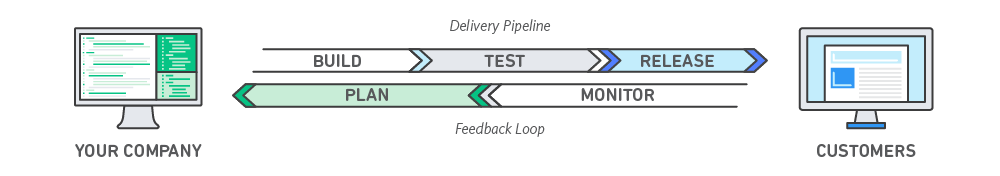
\includegraphics[width=0.8\textwidth]{02-devops.png}
  \caption{Mekanisme DevOps (Sumber:~\cite{devops})}
\end{figure}
DevOps adalah serangkaian filosofi, \textit{practices}, dan kakas yang dapat meningkatkan produktivitas perusahaan, baik secara internal maupun untuk mempercepat proses \textit{delivery} layanan untuk konsumen (\cite{devops}).
Dengan \textit{delivery} yang cepat, tentunya akan dapat berkompetisi dengan lebih efektif di pasar.
Terdapat lima bagian utama dari filosofi DevOps, yaitu \textit{build}, \textit{test}, \textit{release}, \textit{plan}, dan \textit{monitoring}.
Hal yang menjadi tujuan utama untuk DevOps adalah untuk mempercepat dalam proses-proses yang memakan waktu dengan menggunakan otomatisasi yang dapat dilakukan terhadap sistem.

\subsection{\textit{Practices} dalam DevOps}
Terdapat beberapa hal yang menjadi \textit{best practices} dalam DevOps. 
Dalam bagian ini, penulis akan membahas sedikit terkait masing-masing practices yang ada di dalam DevOps yang relevan dengan poin-poin yang ada pada makalah ini.

\begin{enumerate}
  \item Continuous Integration
  
  Continuous Integration (CI) adalah filosofi yang diterapkan dengan tujuan memastikan integritas sistem.
  Biasanya, Continuous Integration dicapai lewat menerapkan \textit{build} dan \textit{test} yang otomatis.
  Continuous Integration akan sangat menunjang TDD (\textit{Test Driven Development}) karena selalu dilakukan secara otomatis setiap kali ada perubahan yang dilakukan kepada sistem.
  Dengan begitu, kualitas sistem, pencarian \textit{bug}, dan penyelesaiannya dapat diselesaikan dengan lebih cepat.

  \item Continuous Delivery
  
  Continuous Delivery (CD) adalah suatu filosofi dengan tujuan untuk memastikan \textit{delivery} dari sistem.
  Dalam konteks ini, \textit{delivery} yang dimaksud adalah melakukan \textit{build} dan \textit{deployment} ke \textit{production} secara otomatis.
  Continuous Delivery juga sangat erat hubungannya dengan continuous Integration, yang terkadang dapat juga dilakukan dalam \textit{pipeline} yang sama.
  Pengaturan \textit{deployment} juga fleksibel, tidak harus melulu untuk \textit{production} saja, walaupun tujuan awalnya untuk melakukan \textit{delivery} dengan cepat.

  \item \textit{Microservices}
  
  \textit{Microservices} adalah sebuah arsitektur untuk sistem, di mana sebuah sistem besar dibuat atas dasar sistem-sistem kecil yang membentuk satu kesatuan besar.
  Secara umum, arsitektur \textit{microservices} dapat memberi dampak positif bagi tim yang besar, karena pengembangan dapat dilakukan secara independen antar sistem, tetapi dari sudut pandang proses \textit{deployment} dilakukan menjadi tidak trivial.
  Meskipun demikian, microservices akan mendukung \textit{scalability} dari sistem ke depannya, dan dengan filosofi DevOps lainnya arsitektur ini sangat baik untuk diterapkan dalam lingkungan pengembangan dengan jumlah pengembang dan tim yang berkembang.

  \item Infrastructure as Code
  
  Infrastructure as Code (IaC) adalah suatu filosofi di mana infrastruktur yang dibuat harus dapat disimpan sebagai program, dengan tujuan memudahkan replikasi dan manajemen infrastruktur sistem.
  Seiring meningkatnya penggunaan sistem berbasis \textit{cloud}, penggunaan Infrastructure as Code juga meningkat karena alasan yang disebut sebelumnya.
  Hal-hal yang dapat dimanajemen lewat Infrastructure as Code meliputi konfigurasi infrastruktur dan policy atau aturan terhadap infrastruktur.
  Dengan kakas-kakas yang ada sekarang, konfigurasi yang ada dapat direalisasikan menjadi infrastruktur yang sesungguhnya.

  \item Monitoring dan Logging
  
  Dalam DevOps, Monitoring dan Logging terhadap sistem menjadi suatu hal yang patut diperhatikan.
  Dengan sistem yang terus berkembang, sistem perlu diawasi untuk memastikan kelancaran dari sistem.
  Sistem dapat diawasi melalui kinerja maupun dan melakukan pengawasan terhadap pencatatan rekam historis dari penggunaan sistem.

\end{enumerate}

\section{GitOps}

% TODO: Possibly buang atau refactor
\todo{Possibly buang atau refactor}

\subsection{Definisi GitOps}

GitOps merupakan sebuah rangka kerja/ \textit{framework} yang menerapkan prinsip DevOps dalam melakukan pengembangan suatu sistem, meliputi penggunaan \textit{version control}, menerapkan CI/CD, dan melakukan otomasi terhadap proses \textit{deployment} sistem\cite{gitlab}. Seringkali, istilah GitOps dibingungkan dengan istilah DevOps, yang pada dasarnya sebenarnya GitOps menerapkan prinsip-prinsip yang ada pada DevOps, dengan memanfaatkan atau menambah kemampuan yang dimiliki dari suatu sistem \textit{version control} seperti git.

Setelah memahami konsep GitOps yang sebenarnya, perlu dipahami komponen yang membentuk GitOps ini. Pada dasarnya, terdapat tiga komponen utama, yaitu: Infrastructure as Code, Merge Request (MR) atau Pull Request (PR), dan Continuous Integration, Continuous Deployment, serta Continuous Delivery (CI/CD).

\subsubsection{Infrastructure as Code}

Dengan perkembangan teknologi yang pesat di masa ini akan sejalan dengan pertumbuhan sistem, mungkin dari suatu perusahaan atau instansi. Seiring bertumbuhnya sistem secara umum tim pengembang sistem juga makin banyak. Terlebih lagi, dengan tren saat ini yang menerapkan penggunaan \textit{microservices} akan membuat sulitnya melakukan manajemen terhadap sistem yang ter-\textit{deploy}, karena tidak mungkin untuk memanajemen server yang jumlahnya tentu tidak sedikit. Belum lagi ketika dipertimbangkan migrasi antar server yang berbeda; belum tentu kedua server disiapkan dengan cara yang sama persis. Hal ini dapat menambah faktor kesalahan manusia yang seharusnya diusahakan untuk dikurangi dalam pengembangan suatu sistem.

Oleh karena itu, salah satu pendekatannya adalah menerapkan \textit{Infrastructure as Code}. \textit{Infrastructure as Code} atau yang sering disebut dengan IaC adalah suatu istilah untuk membuat infrastruktur lewat pembuatan kode. Dengan kode yang sama akan dihasilkan infrastruktur yang identik, sehingga faktor kesalahan manusia dalam \textit{provisioning} manual bisa dikurangi. Sekarang, terdapat beberapa kakas untuk menerapkan IaC seperti Terraform dan Pulumi. 

\subsubsection{Merge Request atau Pull Request}

Merge Request (MR) atau Pull Request (PR) adalah istilah yang umum ditemui di platform berbasis git seperti GitHub dan GitLab. Kedua istilah ini sama; GitLab biasanya menggunakan istilah Merge Request sedangkan GitHub menggunakan istilah Pull Request. Pada dasarnya, mekanisme ini biasanya digunakan untuk memastikan bahwa kode program yang akan digabungkan bisa diperiksa secara terpisah. Selain itu, biasanya MR atau PR bisa ditambahkan pipeline CI/CD untuk melakukan pengujian seperti menggunakan \textit{testing frmaework} atau mungkin menggunakan \textit{linter} untuk menjamin gaya kode yang dibuat. 

\subsubsection{Continuous Integration, Continuous Deployment, dan Continuous Delivery}

Tiga hal ini yang sering disebut dengan CI/CD adalah suatu istilah dalam dunia pengembangan sistem dan perangkat lunak untuk selalu memastikan integritas sistem dan pembawaan perangkat lunak pada pengguna secara terus menerus. Secara teknis, CI/CD pada dasarnya adalah melakukan suatu pekerjaan secara otomatis lewat pembuatan \textit{pipeline} yang memanggil program dalam bentuk apapun dengan tujuan CI/CD tersebut. Beberapa kakas yang populer digunakan saat ini seperti Jenkins, Github Actions, CircleCI, dan masih banyak lagi.

\subsection{Contoh Kakas GitOps}

Contoh kakas yang memanfaatkan prinsip GitOps yang cukup terkenal adalah FluxCD.
Dikutip dari dokumentasi resminya~\cite{fluxcd}, FluxCD adalah kakas yang digunakan untuk memastikan bahwa sebuah cluster Kubernetes tetap tersinkronisasi dengan konfigurasi yang sudah ada pada platform git.
FluxCD juga memanfaatkan API Kubernetes dan memiliki integrasi yang baik dengan kakas umum lainnya yang digunakan dalam sebuah cluster, seperti Prometheus.

Secara umum, fitur yang diberikan oleh FluxCD sudah cukup lengkap dalam menerapkan prinsip GitOps. Fitur-fiturnya tentu meliputi integrasinya dengan Git. Beberapa fitur lainnya adalah integrasi yang baik dengan Helm (kakas untuk melakukan versioning terhadap deployment), memiliki sistem policy validation, role-based access control, manajemen~\textit{dependecy}, dan masih banyak fitur lainnya.
\section{MLOps}

\subsection{Definisi MLOps}

MLOps adalah bagian yang lebih spesifik dari DevOps. 
Seperti yang telah dibahas pada bagian sebelumnya, DevOps adalah suatu metodologi dan prinsip yang diterapkan untuk membuat proses pengembangan sistem menjadi lebih cepat dan efisien. 
MLOps adalah metodologi yang menerapkan DevOps untuk proses-proses yang ada pada pengembangan model machine learning.

Dalam MLOps, terdapat proses-proses tertentu yang spesifik untuk domain pengembangan \textit{pipeline} ML.
Seperti dilansir dari artikel oleh~\cite{mlops}, MLOps ini merupakan bidang yang masih baru karena baru-baru ini teknologi kecerdasan buatan mulai diterapkan dalam perusahaan.
Tujuan dari MLOps adalah untuk melakukan manajemen dari eksperimen dalam proses pengembangan sistem intelijen.
Saat ini, metodologi MLOps juga sudah diterapkan pada berbagai perusahaan besar di dunia, seperti Facebook, Google, AirBnB, dan Uber.

\subsection{Contoh Kakas MLOps}

Di masa lampau, kebutuhan untuk sistem intelijen tidak setinggi di masa kini. 
Oleh karena itu, seperti yang ditulis oleh~\cite{mlops}, perusahaan-perusahaan raksasa seperti Google membuat suatu \textit{framework} internal untuk kebutuhan mereka saat itu.
Seiring meningkatnya keperluan untuk MLOps dalam dunia industri, kakas-kakas MLOps mulai bermunculan.

Kubeflow, seperti tertulis dalam dokumentasi resminya adalah salah satu kakas yang dikembangkan dengan tujuan untuk mempermudah proses \textit{deployment} pada sistem ML dengan mudah.
Seperti namanya, Kubeflow dibuat untuk melakukan \textit{deployment} di atas Kubernetes.
Kubeflow memiliki fitur yang lengkap, seperti adanya TensorFlow dan kakas-kakas ML lainnya, kakas-kakas untuk melakukan eksperimen, menyimpan \textit{hyperparameter}, dan melakukan \textit{model versioning}, serta beberapa aplikasi yang digunakan untuk melakukan monitoring di Kubernetes juga, seperti Prometheus.
Dengan dibangunnya Kubeflow di atas Kubernetes, hal itu membuat melakukan  \textit{deployment} pada \textit{platform-platform} berbasis \textit{cloud} menjadi mudah.


\section{Masalah Umum}

Dilansir dari beberapa sumber, terdapat beberapa masalah yang sering dihadapi dalam penerapan prinsip GitOps dan \textit{Infrastructure as Code}, meliputi:

\begin{itemize}
  \item Tidak menjamin bahwa \textit{provisioning} yang dilakukan menjamin penerapan prinsip-prinsip yang baik dalam pengembangan sistem.
  \item Melakukan manajemen sistem yang \textit{multirepo} serta melakukan \textit{deployment}-nya.
  \item Sulitnya melakukan audit terhadap perubahan sistem dengan kemungkinan sistem yang bisa berubah dengan cepat.
\end{itemize}


\section{Masalah Keamanan di Infrastructure as Code}

% TODO: Possibly buang atau refactor
\todo{Possibly buang atau refactor}

Bagian ini akan membahas masalah-masalah keamanan yang sering ditemui ketika memanfaatkan prinsip Infrastructure as Code, serta sedikit terkait penanganannya. Bagian ini secara khusus mengutip laporan yang dibuat oleh~\cite{8812041}. Laporan tersebut dibuat dengan mengumpulkan data-data dari banyak kode program dan menandai masalah-masalah yang umum terjadi.

\subsection{User Admin Secara Bawaan}
Banyak sekali yang menggunakan user admin secara bawaan, tanpa membuat user baru dengan batasan yang sesuai. Tentunya ini akan menimbulkan masalah keamanan ke depannya bila user tersebut bocor. Walaupun sederhana, seharusnya perlu dibuat suatu user dengan akses yang seminimal mungkin.

\subsection{Pemberian Kata Sandi Kosong}
Kata sandi dalam program IaC seringkali dikosongkan untuk kemudahan dalam pengembangan. Terkadang, hal tersebut dilupakan dan sampai di production. Tentunya bukan hal yang baik dan hal ini tentunya dapat mempermudah orang lain untuk menerka kata sandi tersebut. Seminimalnya, isi kata sandi dengan suatu string; jangan sampai kata sandi benar-benar kosong.

\subsection{Adanya~\textit{Hard-coded Secrets}}
Serupa dengan pemberian kata sandi yang kosong, biasanya hard-coded secrets ini terjadi akibat demi mempermudah proses pengembangan. Untuk melakukan uji coba, hal-hal seperti kata sandi dimasukkan secara plainteks di kode yang dibuat dan terlupa untuk diganti di production. Dalan laporan tersebut, hal-hal yang diperiksa meliputi username, private key, dan kata sandi. Walau begitu, ada kasus di mana hal seperti ini memang diperlukan, namun hal ini menimbulkan pertanyaan dan potensi bahaya secara keamanan

\subsection{Binding IP Address yang Kurang Tepat}
Masalah ini biasanya timbul dalam proses pengembangan juga. Umumnya, kesalahan ini muncul karena menggunakan alamat 0.0.0.0 yang terbuka. Walau belum tentu menjadi masalah, bisa jadi hal ini menimbulkan masalah keamanan.

\subsection{Komentar Mencurigakan dalam Kode}
Komentar mencurigakan yang dimaksud adalah menandai suatu bagian program dengan TODO, FIXME, dan hal-hal serupa. Biasanya, hal ini bisa menandakan bahwa ada hal yang tidak diimplementasikan dengan tepat. Memang belum tentu seperti itu, namun dalam laporan yang diberikan ini bisa menjadi masalah keamanan ke depannya.

\subsection{Menggunakan HTTP tanpa TLS}
Seperti yang sudah diketahui, HTTP bukanlah protokol yang aman, sehingga disarankan untu pembuat layanan menggunakan HTTP dengan TLS atau HTTPS. HTTPS lebih aman dibandingkan HTTP karena ada TLS yang melakukan encryption handshake. Walau begitu, HTTP masih sering digunakan walaupun tidak aman, sehingga ini termasuk dalam masalah keamanan yang ditemui dalam kode \textit{Infrastructure as Code}.

\subsection{Menggunakan Algoritma Kriptografi yang Lemah}
Walaupun sudah diberi password, terkadang algoritma kriptografi yang digunakan adalah algoritma kriptografi yang lemah atau sudah ditemukan celah keamanannya, seperti algoritma MD5. Hal ini juga termasuk salah satu dari tujuh hal yang sering ditemui menjadi masalah.




\section{Otomatisasi}\label{automation}

Dalam bagian ini, akan dibahas terkait prinsip dan konsep yang secara umum diterapkan dalam melakukan otomatisasi sistem. Selain itu, akan dibahas terkait aspek apa saja dari sebuah sistem yang diotomatisasi. Hal yang akan dibahas pada bagian ini adalah hal-hal yang sudah terbukti efektif untuk diotomatisasi.

\subsection{Alasan Melakukan Otomatisasi}
Otomatisasi di masa ini menjadi hal yang diusahakan oleh tim pengembang sistem dan perangkat lunak, terutama pada tim yang besar. Walaupun begitu, terkadang otomatisasi menjadi hal yang dikesampingkan dalam proses pengembangan, yang seharusnya dapat mengingkatkan produktivitas pengembangan.

Pada sub bagian ini, penulis akan membahas terkait beberapa alasan untuk melakukan otomatisasi (\cite{beyer2016site}), yaitu sebagai berikut:

\begin{itemize}
  \item Menetapkan konsistensi dalam melakukan pekerjaan yang repetitif
  \item Memusatkan titik kesalahan dalam pengembangan sistem
  \item Mempercepat proses perbaikan sistem
  \item Memperkecil waktu aksi untuk melakukan suatu kegiatan terkait infrastruktur
  \item Menghemat waktu secara umum
\end{itemize}

Dalam otomatisasi, tentunya konsistensi bisa ditetapkan secara internal dengan asumsi faktor eksternal di luar dari kode sistem tidak ada masalah. Otomatisasi yang seharusnya dilakukan hanya melakukan satu hal saja secara konsisten. Bila terjadi masalah di luar fungsionalitas internal sistem, kemungkinan besar masalah tersebut berasal dari faktor eksternal.

Dengan melakukan otomatisasi juga, secara umum tim-tim menggunakan satu platform. Tentu tujuannya untuk mempermudah tim dalam melakukan otomatisasi, sehingga semuanya serba terpusat pada platform tersebut. Hal ini membawa dampak positif juga, karena semua masalah bisa ditelusuri dari platform tersebut.

Perbaikan sistem menjadi hal umum yang dilakukan di setiap proses pengembangan. Oleh karena itu, otomatisasi tentunya dapat membantu proses perbaikan agar lebih efisien, sehingga waktu ynag tersisa bisa digunakan untuk tugas atau kegiatan lain yang lebih produktif untuk pengembangan sistem.

Seperti dituliskan sebelumnya, mengurangi kegiatan yang repetitif dengan otomatisasi bisa menambah waktu untuk pengembangan sistem. Dalam kata lain, aksi-aksi tertentu juga dapat dilakukan lebih cepat lewat proses otomatisasi ini. Tentu saja, salah satu tujuan utamanya untuk menghemat waktu dari proses pengembangan ini. Walaupun mungkin tidak begitu terasa di awal dan mungkin malah menambah \textit{overhead} dalam proses awal pengembangan, semakin lama nilai yang didapatkan dari otomatisasi semakin besar.

\subsection{Aspek Otomatisasi}
Dalam bagian ini tidak akan dibahas secara menyeluruh terkait aspek apa saja yang dapat diotomatisasi, karena pada dasarnya apapun bisa diotomatisasi dalam sebuah sistem, namun dampak yang diberikan bisa jadi belum tentu positif. Oleh karena itu, pada bagian ini aspek-aspek yang sudah terbukti.

Beberapa hal yang bisa dilakukan seputar otomatisasi sistem adalah sebagai berikut (\cite{beyer2016site}):
\begin{itemize}
  \item Pembuatan user account baru
  \item Melakukan turnup dan turndown pada sebuah layanan di cluster
  \item Melakukan rilis versi baru
  \item Menginstall software dengan versi yang lebih baru
\end{itemize}

Tentunya, masih banyak hal yang bisa diotomatisasi. Daftar tersebut hanya daftar singkat dari apa yang bisa diotomatisasi dari sistem secara umum. 
Perlu kita ingat bahwa otomatisasi yang dilakukan belum tentu efektif, sehingga kita perlu mengujinya secara langsung untuk melihat apakah \textit{feasible} untuk melakukan hal tersebut.
Masalah-masalah yang ada dalam sebuah sistem dapat menjadi pedoman untuk membuat otomatisasi pada sistem lewat teknologi-teknologi yang ada.

\section{Potensi Otomatisasi dalam MLOps}

Seperti yang telah dibahas pada bagian sebelumnya, MLOps terdiri dari tiga tahapan utama, yaitu Data Engineering, Model Engineering, dan Code Engineering.
Dalam praktiknya, bagian yang merupakan \textit{toil} dalam ketiga proses ini berada paling banyak dalam tahap data engineering.
Preprocessing dan eksplorasi data umumnya perlu butuh waktu yang lama karena melibatkan beberapa domain dan beberapa faktor lainnya.
Sehingga, perlu metodologi tertentu untuk membantu dalam proses preprocessing data baik secara infrastruktur dan metode pemrosesannya.

Selain tahap tersebut, dalam tahap lain juga terdapat potensi untuk melakukan otomatisasi.
Di masa ini, banyak kakas-kakas yang tersedia untuk membantu dalam proses MLOps.
Contohnya, dalam Kubeflow terdapat fitur melakukan pipelining untuk melakukan proses-proses tertentu dalam langkah yang berbeda-beda.
  \clearpage
\chapter{Kakas Konversi Eksperimen Pemelajaran Mesin untuk Kode Sistem}\label{chap:3}

\section{Analisis Masalah}

Saat ini, konversi dari eksperimen ke sistem yang \textit{production-ready} masih dilakukan secara manual.
Dari ekperimen tersebut, biasanya terdapat proses-proses untuk melakukan pemrosesan data.
Pemrosesan data dapat dilakukan secara langsung sebelum dimasukkan ke dalam model, ataupun dilakukan prekomputasi untuk mempercepat proses inferensi dengan mengabaikan faktor masukan data.
Dalam percobaan-percobaan yang memanfaatkan teknologi seperti Kubeflow, dapat digunakan sistem \textit{pipeline} yang tersedia untuk melakukan eksperimentasi.

Dengan penggunaan \textit{pipeline} dalam eksperimen pemelajaran mesin, proses eksperimen dapat dilakukan dengan lebih cepat.
Hal tersebut karena \textit{pipeline} didesain agar dapat digunakan kembali di beberapa proses yang serupa.
Proses yang dirujuk dapat berupa proses untuk melakukan pemrosesan pada data, atau dapat untuk melakukan proses pelatihan model.
Pembuatannya yang membutuhkan script Python secara umum membuat proses pada \textit{pipeline} ini bersifat atomik serta fleksibel untuk digunakan dalam pelatihan model yang berbeda.

Sejauh dari hasil pencarian penulis, penggunaan \textit{pipeline} ini biasanya sebatas  untuk digunakan dalam eksperimen saja.
Pipeline yang dibuat untuk eksperimen ini biasanya tidak digunakan lagi dalam proses pembuatan sistem inferensi, karena hasil eksperimen biasanya akan disimpan dalam sebuah file yang hanya perlu dibungkus lewat suatu metode komunikasi, seperti yang telah dibahas pada bagian~\ref{chap:model-serving}.
Dengan penggunaan \textit{pipeline} ini ada kemungkinan proses pembuatan sistem dapat dilakukan secara lebih mulus.
Pipeline yang didefinisikan dapat membantu untuk membangun bagian-bagian kecil dari sistem khususnya dalam pemrosesan data. 

Selain itu, model hasil eksperimen yang sukses biasanya hanya hanya perlu untuk dibungkus dalam sebuah metode komunikasi sesuai dengan kebutuhan arsitektur, misalnya dengan gRPC atau REST.\@
Perlu adanya perjanjian antar sistem untuk memastikan objek yang dikirim dan diterima sesuai dengan pihak yang membutuhkan sistem.
Misalnya, seperti dalam gRPC yang menggunakan Protobuf terdapat konvensi perjanjian prosedur dan struktur data yang terlibat, atau JSON Schema dan Swagger dalam REST.\@

\section{Solusi Umum}

Seperti yang disinggung sebelumnya, konversi eksperimen masih relatif manual dan belum memanfaatkan pipeline yang ada.
Sehingga, terdapat potensi pengembangan untuk membuat suatu kakas yang bisa mengubah eksperimen menjadi sistem yang siap digunakan secara sudut pandang pengembangan perangkat lunak.
Berdasarkan eksperimen yang dilakukan lewat pipeline, secara teori memungkinkan untuk mengubah komponen-komponen yang ada dalam pipeline tersebut menjadi beberapa bagian dalam suatu sistem.
Solusi yang dibuat dapat memperhatikan juga struktur data dan prosedur sehingga masukan, keluaran, dan prosedur yang ada dalam sistem bisa terjamin.

Dalam sistem pembelajaran mesin, masukan data diberikan secara mentah tanpa pemrosesan apapun, tetapi terkadang terdapat data yang berbeda sehinga perlu dilakukan pemrosesan yang berbeda.
Pipeline yang sudah ada dalam membuat suatu alur pemrosesan data di dalam sistem dapat dimanfaatkan.
Bila diimplementasikan secara modular, untuk beberapa hal mungkin juga digunakan bahasa yang lebih cepat, sehingga hanya proses inferensi model saja dan beberapa hal saja yang sulit untuk dipindahkan ke bahasa lain.

Sebagai contoh, dalam pemrosesan data tabular umumnya terdapat beberapa tahapan dalam melakukan pemrosesan terhadap data.
Tahapan \textit{preprocessing} dapat berupa normalisasi terhadap fitur, pembentukan fitur baru, seleksi fitur, dan transformasi fitur.
Seperti pada transformasi fitur yang menggunakan metode seperti \textit{Principal Component Analysis} (PCA) atau \textit{Linear Discriminant Analysis} (LDA), tentunya akan memerlukan proses konversi dari data mentah menjadi data dengan dimensi yang berbeda.

\section{Kakas Konversi Eksperimen Pemelajaran Mesin untuk Kode Sistem}

\begin{figure}[ht]
  \centering
  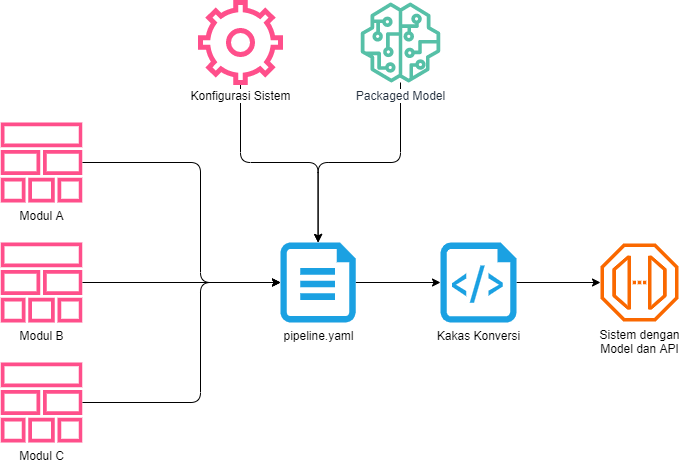
\includegraphics[width=0.7\textwidth]{03-rancangan-solusi.drawio.png}
  \caption{Rancangan Solusi Konversi Eksperimen}\label{fig:03-tool}
\end{figure}

Dalam tugas akhir ini, dibuat suatu prototipe kakas yang penulis sebut sebagai \monospace{myx} yang menggunakan hasil eksperimen yang selesai digunakan menjadi kode sistem yang siap digunakan (lihat Gambar~\ref{fig:03-tool}).
Definisi dari perjanjian data yang menjadi masukan dan keluaran akan dibuat oleh sistem secara otomatis berdasarkan eksperimen.
Alur pemrosesan yang didefinisikan dapat dibuat lewat \textit{markup file} seperti JSON atau YAML yang formatnya sudah ditentukan untuk kakas tersebut.
Alur didefinisikan lewat pemanggilan modul-modul yang diimplementasikan lebih dulu yang nantinya dapat memanggil sebuah model yang biasanya sudah siap dan disimpan dalam sebuah file.
Rincian mengenai implementasi kakas ini dapat dilihat pada Lampiran~\ref{appendix:srs}.

Selain dari konfigurasi yang didefinisikan, untuk menjalankan kakas diperlukan juga \textit{file-file} eksperimen terkait.
\textit{File-file} eksperimen yang dimaksud salah satunya adalah model hasil eksperimen.
Selain itu, \textit{file-file} eksperimen juga dapat berupa \textit{file} hasil dari eksperimen yang digunakan untuk melakukan transformasi terhadap data, misalnya seperti \textit{scaler} atau \textit{encoder} dalam eksperimen data tabular.

Modul yang dimaksud berupa potongan program yang siap untuk disatukan dengan potongan program lainnya untuk membentuk suatu sistem yang berjalan.
Modul dapat diimplementasikan dalam bahasa apapun selama semua modul yang digunakan menggunakan bahasa yang sama.
Dalam pendekatan yang umum, digunakan Docker sebagai bantuan untuk melakukan pemrosesan terhadap data.
Metode ini diterapkan dalam pengembangan eksperimen yang iteratif.
Dalam pengembangan sistem pemelajaran mesin, hal ini menjadi kurang baik karena akan memerlukan komputasi yang lebih berat akibat penggunaan \textit{containerization} yang pada dasarnya tidak diperlukan.

Hasil akhir dari kakas ini adalah sebuah kode sistem yang siap digunakan untuk \textit{production} yang terbentuk dari konfigurasi masukan seperti modul-modul yang dinginkan.
Kakas ini bersifat \textit{non-domain specific} atau dapat digunakan untuk kasus pembuatan sistem inferensi secara umum.
Pemilihan \textit{interface} untuk model ditentukan lewat \textit{markup file} yang telah dibuat.
Metode komunikasi yang akan diimplementasikan adalah REST sebagai contoh dari \textit{interface} yang umum digunakan dalam sistem.

Penulis mengimplementasikan kakas ini dalam bahasa Go.
Pemilihan bahasa didasarkan kepada \textit{library} yang tersedia dalam bahasa tersebut dan bahasa Go yang bersifat \textit{strong-typing} untuk memastikan struktur program yang baik.
Hasil dari proses konversi yang dilakukan kakas akan berupa kode program dalam bahasa Python dengan \monospace{FastAPI}.


\section{Format Konfigurasi}

Seperti yang disinggung pada bagian sebelumnya, kakas ini akan menerima masukan berupa \textit{markup file} yang menjadi konfigurasi dari sistem.
\textit{File} ini tentunya mengandung pengaturan yang diperlukan dalam membangun suatu kode sistem.
Beberapa hal yang terdapat dari konfigurasi berdasarkan pertimbangan penulis untuk menyelesaikan masalah adalah sebagai berikut:

\begin{enumerate}
	\item Format masukan
	\item Format keluaran
	\item Format model
	\item Alur pemrosesan
	\item \textit{Interface} yang disediakan
\end{enumerate}

Sebagai catatan, format masukan dan keluaran yang dimaksudkan adalah untuk pengunaan sistem secara \textit{interface} dan bukan untuk model yang menjadi bagian dari sistem.
Dalam bagian ini, akan dibahas mengenai komponen untuk 

\subsection{Konfigurasi Format Masukan}

Sistem pemelajaran mesin saat ini memiliki banyak bentuk masukan.
Salah satu bentuk masukan yang umum digunakan adalah bentuk yang berupa tabel atau tabular.
Format masukan perlu didefinisikan untuk membantu dalam proses pembuatan kode khususnya terkait dengan \textit{interface}.
Berikut adalah contoh konfigurasi untuk bagian masukan sistem yang berupa data tabular:

\yamlcode{resources/files/configurations/input_basic.yml}

Mengingat jenis masukan bisa beragam, tidak menutup kemungkinan masukan dengan bentuk lain bisa digunakan dalam model, contohnya seperti masukan yang berupa gambar.
Masukan gambar memiliki aturan-aturan seperti layaknya data tabular, seperti panjang dan lebar dari sebuah gambar.
Berikut adalah contoh konfigurasi untuk masukan yang berupa data gambar:

\yamlcode{resources/files/configurations/input_image.yml}

Selain dari format masukan yang beragam, terkadang masukan kepada sistem bisa berbeda dengan masukan pada model.
Alasan dari perbedaan tersebut adalah terdapat pemrosesan data yang dilakukan oleh sistem untuk membuat masukan pada sistem lebih intuitif.
Oleh karena itu, konfigurasi dari format masukan juga perlu menangani hal tersebut.
Berikut adalah contoh konfigurasi untuk masukan yang perlu dilakukan pemrosesan data:

\yamlcode{resources/files/configurations/input_preprocessed.yml}

\subsection{Konfigurasi Format Keluaran}
Serupa dengan bagaimana format masukan didefinisikan, format keluaran perlu didefinisikan juga.
Format keluaran tidak memiliki variasi lebih banyak dari format masukan.
Format keluaran bergantung dari domain permasalahan serta teknik-teknik pembelajaran mesin yang digunakan.
Misalnya, dalam permasalahan klasifikasi format keluaran akan berupa sekumpulan prediksi dari model yang mungkin disertai dengan derajat kepercayaan dari prediksi tersebut.
Permasalahan regresi juga akan mengembalikan suatu nilai numerik.
Tidak sebatas dalam teknik-teknik \textit{supervised} saja, teknik \textit{unsupervised} seperti \textit{clustering} yang memiliki keluaran yang serupa dengan klasifikasi.
Berikut adalah contoh konfigurasi untuk keluaran sederhana:

\yamlcode{resources/files/configurations/output_basic.yml}

\subsection{Konfigurasi Format Model}
Eksperimen untuk membuat model pembelajaran mesin menerapkan penggunaan banyak kakas-kakas bantuan yang umum digunakan, seperti Tensorflow, SKLearn, Catboost, dan banyak kakas-kakas lainnya.
Akibat kakas-kakas yang beragam, secara umum model yang telah dilatih akan disimpan dalam sebuah \textit{file} dengan format ekstensi tertentu.
Format yang penulis pilih adalah format ONNX (Open Neural Network Exchange) karena memiliki banyak integrasi dengan kakas-kakas yang bermacam-macam jenisnya.
ONNX juga memiliki kemampuan untuk melakukan inferensi dengan cara yang seragam untuk kakas-kakas yang berbeda jenis.

Walaupun begitu, tidak menutup kemungkinan untuk konfigurasi tidak menggunakan format lain.
Misalnya, pada kakas Tensorflow disediakan sebuah cara untuk menyimpan model dalam sebuah file lewat \mintinline{python}{save_model()}.
Oleh karena itu, konfigurasi format model harus bisa menerima jenis model yang berbeda-beda.
Berikut ini adalah contoh konfigurasi sederhana untuk format model

\subsection{Konfigurasi Alur Pemrosesan}
Secara umum, terkadang perlu tahapan-tahapan tertentu dari masukan yang diberikan terhadap sistem.
Misalnya, dalam data tabular kadang dilakukan proses \textit{scaling} terhadap data atau melakukan reduksi dimensi dengan menggunakan teknik seperti PCA dan LDA.
Masukan berupa gambar kadang diperlukan untuk melakukan tahap \textit{image processing} untuk memastikan gambar yang dimasukkan cocok untuk sistem.
Kakas ini akan menerima konfigurasi untuk melakukan hal-hal tersebut lewat modul-modul yang didefinisikan dalam konfigurasi.

\subsection{Konfigurasi \textit{Interface}}
Sistem secara umum akan menggunakan salah satu atau kedua dari \textit{interface}, yaitu REST atau gRPC.
Dengan mempertimbangkan kedua hal tersebut, kakas ini akan berfokus pada kedua \textit{interface} tersebut.
Kode dari sistem yang dibangkitkan tentunya dapat dimodifikasi sesuai kebutuhan dari sistem bila diperlukan perubahan terhadap \textit{interface}.

  
  % bibliography
  \addcontentsline{toc}{chapter}{Daftar Pustaka}
\printbibliography[title={Daftar Pustaka}]

\end{document}
